\chapter{Rework}
\label{rework}


Flux is your friend when doing rework.  However, you need to remove it
from your board when finished, see \hyperref[flux removal]{flux
  removal}.  You should check all rework with a magnifier and look for
solder bridges.


\section{Removing resistors and capacitors}

\begin{enumerate}
\item Apply flux from syringe to pads.

\item Use tweezer soldering iron.
\end{enumerate}


\section{Removing larger parts}


\begin{enumerate}
\item Apply flux from syringe to pads.

\item Use a grunty soldering iron.  \textbf{Do not push hard with a
  small soldering iron since this will bend the tips.}
\end{enumerate}



\section{Removing MCU}

\begin{enumerate}
\item Only remove as last resort.

\item Apply flux from syringe to all pins.

\item Get Scott to show you how to use the hot-air gun.  The key is to
  choose a head that matches the size of the MCU and getting the
  temperature correct.

\item Be careful not to lift pads or tracks.
\end{enumerate}



\section{Adding a wire}

\begin{enumerate}
\item For a signal trace, choose the very fine wire.

\item Cut to length and strip insulation from both ends.  The second
  end is a lot harder!

\item Bend wire to shape and tape down to the PCB.  Note, you can run
  this wire through vias.

\item Apply flux from syringe to both pads.

\item Use small soldering iron to solder wires in place.
\end{enumerate}


\section{Flux removal}

\begin{enumerate}
\item Scrub board with using flux-cleaner and brush.
\item Clean board with a towel.
\item Wash board with a little bit of IPA.
\item Clean board with a towel.
\end{enumerate}


\mtodo{Show photos of clean board and dirty board}


\begin{figure}[!h]
  \centering 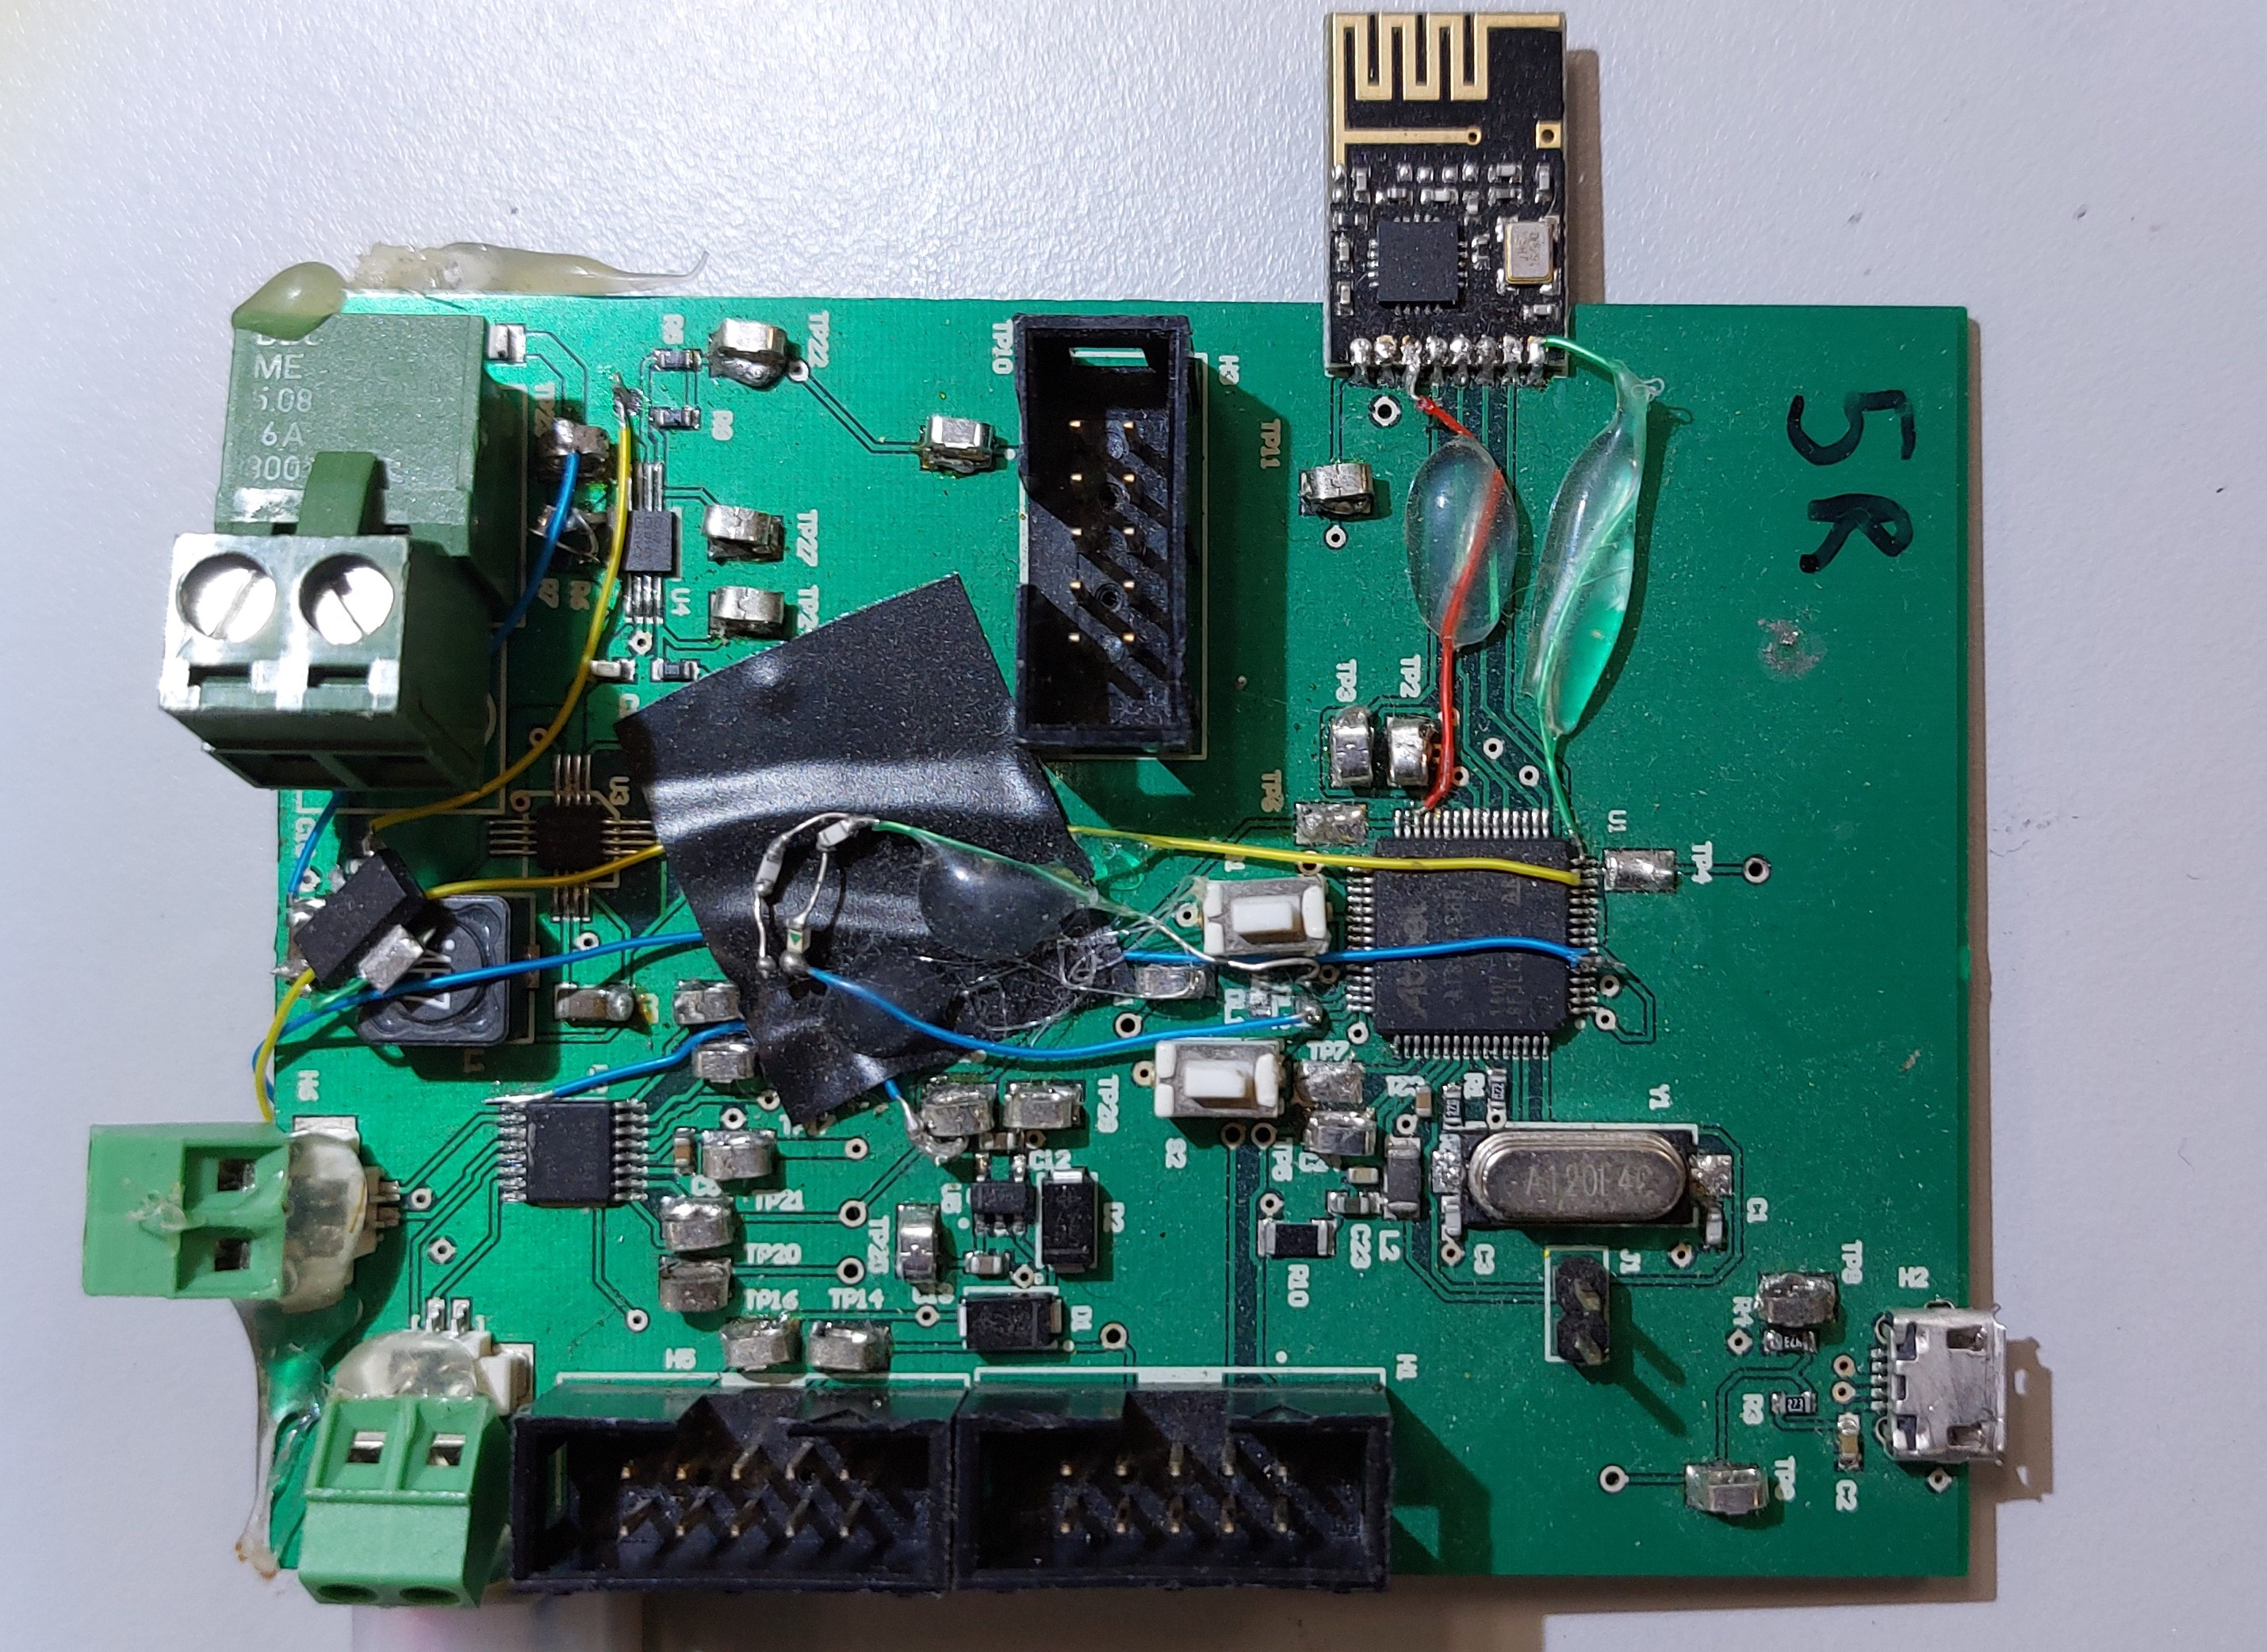
\includegraphics[width=6in]{figs/rework2.jpg}
  \caption{Example of a PCB where not much care was taken with the
    schematic resulting in a lot of rework. The board worked!}
  \label{fig:rework2}
\end{figure}
